\documentclass[10pt]{article}
\usepackage{fullpage,enumitem,amsmath,amssymb,graphicx,listings,tikz,bbm,xcolor}
\setlength{\parindent}{0pt}

\begin{document}

\begin{center}
{\Large \textbf{Homework 8: From Language to Logic}}

\begin{tabular}{rl}
\\
Course: & CS 221 Spring 2019 \\
Name: & Bryan Yaggi
\end{tabular}
\end{center}

In this assignment, you will get some hands-on experience with logic. You'll see how logic can be used to represent the meaning of natural language sentences, and how it can be used to solve puzzles and prove theorems. Most of this assignment will be translating English into logical formulas, but in Problem 4, we will delve into the mechanics of logical inference.

\section*{\normalsize Problem 1: Propositional Logic}

\begin{enumerate}[label=(\alph*)]

	\item coding
	
	\item coding
	
	\item coding

\end{enumerate}

\section*{\normalsize Problem 2: First-Order Logic}

\begin{enumerate}[label=(\alph*)]

  \item coding
  
  \item coding
  
  \item coding
  
  \item coding

\end{enumerate}

\section*{\normalsize Problem 3: Liar Puzzle}

\begin{enumerate}[label=(\alph*)]

  \item coding

\end{enumerate}

\section*{\normalsize Problem 4: Logical Inference}

Having obtained some intuition on how to construct formulas, we will now perform logical inference to derive new formulas from old ones. Recall that:
\begin{itemize}

	\item Modus ponens asserts that if we have two formulas, $A \rightarrow B$ and $A$ in our knowledge base, then we can derive $B$.
	
	\item Resolution asserts that if we have two formulas, $A \vee B$ and $\neg B \vee C$ in our knowledge base, then we can derive $A \vee C$.
	
	\item If $A \wedge B$ is in the knowledge base, then we can derive both $A$ and $B$. 
	
\end{itemize}

\begin{enumerate}[label=(\alph*)]

  \item Some inferences that might look like they're outside the scope of Modus ponens are actually within reach. Suppose the knowledge base contains the following two formulas:
  $$KB = \{ (A \vee B) \rightarrow C, A \}$$
  Your task: First, convert the knowledge base into conjunctive normal form (CNF). Then apply Modus ponens to derive $C$. Please show how your knowledge base changes as you apply derivation rules.
  
  Hint: You may use the fact that $P \rightarrow Q$ is equivalent $\neg P \vee Q$.
  
  Remember, this isn't about you as a human being able to arrive at the conclusion, but rather about the rote application of a small set of transformations (which a computer could execute).
  
  \begin{align*}
  KB &= \{ (A \vee B) \rightarrow C, A \}\\
  KB &= \{ \neg (A \vee B) \vee C, A \}\\
  KB &= \{ (\neg A \wedge \neg B) \vee C, A \}\\
  KB &= \{ (\neg A \vee C) \wedge (\neg B \vee C), A \}\\
  KB &= \{ \neg A \vee C, \neg B \vee C, A \} &\textit{CNF}\\
  KB &= \{ A \rightarrow C, B \rightarrow C, A \}\\
  &\frac{A, A \rightarrow C}{C} &\textit{modus ponens}
  \end{align*}
  
  \item Recall that Modus ponens is not complete, meaning that we can't use it to derive everything that's true. Suppose the knowledge base contains the following formulas:
  $$KB = \{ A \vee B, B \rightarrow C, (A \vee C) \rightarrow D \}$$
  In this example, Modus ponens cannot be used to derive $D$, even though $D$ is entailed by the knowledge base. However, recall that the resolution rule is complete.
  
  Your task: Convert the knowledge base into CNF and apply the resolution rule repeatedly to derive $D$.
  
  \begin{align*}
  KB &= \{ A \vee B, B \rightarrow C, (A \vee C) \rightarrow D \}\\
  KB &= \{ A \vee B, \neg B \vee C, \neg A \vee D, \neg C \vee D \} &\textit{CNF}
  \end{align*}
  
  \begin{center}
	  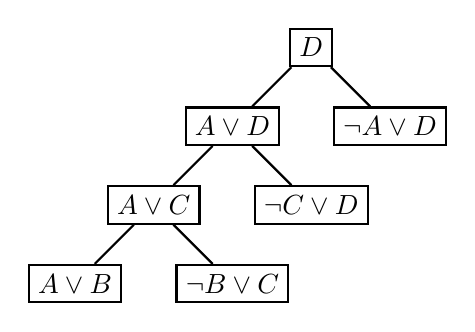
\begin{tikzpicture}
			\begin{scope}[every node/.style={rectangle,thick,draw}]
				\node (f1) at (0,0)	 {$D$};  		
	    		\node (f2) at (-1,-1) {$A \vee D$};
	    		\node (f3) at (1,-1) {$\neg A \vee D$};
	    		\node (f4) at (-2,-2) {$A \vee C$};
	    		\node (f5) at (0,-2) {$\neg C \vee D$};
	    		\node (f6) at (-3,-3) {$A \vee B$};
	    		\node (f7) at (-1,-3) {$\neg B \vee C$};
			\end{scope}
			\begin{scope}[every edge/.style={draw=black,thick}]
				\path [-] (f1) edge node {} (f2);	    		
	    		\path [-] (f1) edge node {} (f3);
	    		\path [-] (f2) edge node {} (f4);	    		
	    		\path [-] (f2) edge node {} (f5);
	    		\path [-] (f4) edge node {} (f6);	    		
	    		\path [-] (f4) edge node {} (f7);
			\end{scope}
		\end{tikzpicture}
	\end{center}

\end{enumerate}

\section*{\normalsize Problem 5: Odd and Even Integers}

In this problem, we will see how to use logic to automatically prove mathematical theorems. We will focus on encoding the theorem and leave the proving part to the logical inference algorithm. Here is the theorem:\smallskip

If the following constraints hold:

\begin{itemize}
	\item Each number $x$ has exactly one successor, which is not equal to $x$.
	\item Each number is either odd or even, but not both.
	\item The successor of an even number is odd.
	\item The successor of an odd number is even.
	\item For every number $x$, the successor of $x$ is larger than $x$.
	\item Larger is a transitive property: if $x$ is larger than $y$ and $y$ is larger than $z$, then $x$ is larger than $z$. 
\end{itemize}

Then we have the following consequence:

\begin{itemize}
	\item For each number, there is an even number larger than it.
\end{itemize}

Note: in this problem, "larger than" is just an arbitrary relation, and you should not assume it has any prior meaning. In other words, don't assume things like "a number can't be larger than itself" unless explicitly stated.

\begin{enumerate}[label=(\alph*)]

  \item coding
  
  \item Suppose we added another constraint:
  \begin{itemize}
		\item A number is not larger than itself.
	\end{itemize}
	Prove that there is no finite, non-empty model for which the resulting set of 7 constraints is consistent. This means that if we try to prove this theorem by model checking only finite models, we will find that it is false, when in fact the theorem is true for a countably infinite model (where the objects in the model are the numbers).
	
	Consider the set $x = \{ x_1, x_2, x_3, \dots, x_n \}$\\
	Given constraints 1, 5, and 6, $x$ would be consistent if $x_1 < x_2 < x_3 < \dots < x_n$ and $x_n < x_1$.\\
	When the last constraint is added, $x$ is not consistent because the cycle is no longer valid since $x_1 < x_1 = false$.
  
\end{enumerate}

\end{document}
